%----------------------------------------------------------------------------------------
%	PACKAGES AND OTHER DOCUMENT CONFIGURATIONS
%----------------------------------------------------------------------------------------

\documentclass[paper=a4, fontsize=11pt]{scrartcl} % A4 paper and 11pt font size

\usepackage{fourier} % Use the Adobe Utopia font for the document - comment this line to return to the LaTeX default
\usepackage[utf8]{inputenc}
\usepackage[french]{babel}
\usepackage{amsmath,amsfonts,amsthm} % Math packages
\usepackage{graphicx}


\usepackage{lipsum} % Used for inserting dummy 'Lorem ipsum' text into the template

\usepackage{sectsty} % Allows customizing section commands
\allsectionsfont{\centering \normalfont\scshape} % Make all sections centered, the default font and small caps

%\usepackage{fancyhdr} % Custom headers and footers
%\pagestyle{fancyplain} % Makes all pages in the document conform to the custom headers and footers
%\fancyhead{} % No page header - if you want one, create it in the same way as the footers below
%\fancyfoot[L]{} % Empty left footer
%\fancyfoot[C]{} % Empty center footer
%\fancyfoot[R]{\thepage} % Page numbering for right footer
%\renewcommand{\headrulewidth}{0pt} % Remove header underlines
%\renewcommand{\footrulewidth}{0pt} % Remove footer underlines
%\setlength{\headheight}{13.6pt} % Customize the height of the header
%\setlength\parindent{0pt} % Removes all indentation from paragraphs - comment this line for an assignment with lots of text

%----------------------------------------------------------------------------------------
%	TITLE SECTION
%----------------------------------------------------------------------------------------

\newcommand{\horrule}[1]{\rule{\linewidth}{#1}} % Create horizontal rule command with 1 argument of height

\title{
\normalfont \normalsize
\textsc{Ensimag - Algorithmique et Optimisation Discrète} \\ [25pt] % Your university, school and/or department name(s)
\horrule{0.5pt} \\[0.4cm] % Thin top horizontal rule
\huge Distance de Fréchet \\ % The assignment title
\horrule{2pt} \\[0.5cm] % Thick bottom horizontal rule
}

\author{Pierre Bouvier, Maxime Gourgoulhon} % Your name

\date{\normalsize\today} % Today's date or a custom date
\usepackage[margin=0.5in]{geometry}
\begin{document}

%\maketitle % Print the title

%----------------------------------------------------------------------------------------
%	PROBLEM 1
%----------------------------------------------------------------------------------------

\section*{AOD - Distance de Fréchet}
Gourgoulhon Maxime et Bouvier Pierre


\subsection*{Question 5 - Programmation dynamique}

Voir frechet.c
%------------------------------------------------


\subsection*{Question 6 - Analyse Théorique}

L'algorithme utilisé est récursif et itératif : il est est récursif jusqu'à un certain seuil, puis itératif. Il s'agit d'un algorithme de type "cache-oblivious".
Voir le schéma :

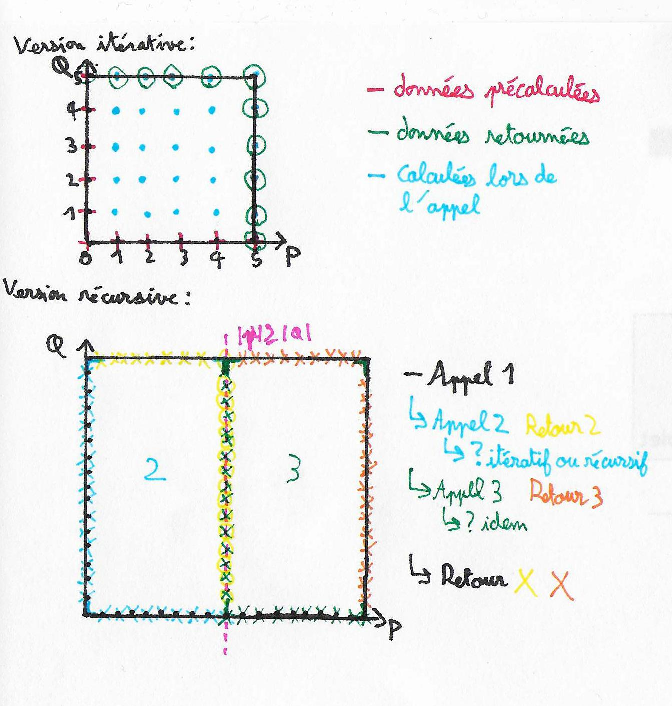
\includegraphics[]{scan.pdf}

Au niveau de l'implémentation, les chemins sont représentés par des listes chaînées.
%Chaque point du schéma est une structure contenant la distance de Fréchet jusqu'à ce point
L'implémentation a l'avantage d'être économe en mémoire.

La version itérative reçoit les deux chemins du fichier d'entrée, avec les deux points départ et arrivé, ainsi que les tableau précalculés et un pointeur vers le résultat.

La fonction itérative a un coût asymptotique en nombre d'opération (se trouve dans la boucle principale : 12,67 instructions en moyenne) : $ (Max_p - Min_p) * (Max_q - Min_q) = n^2$

Le coût asymptotique en espace mémoire lors de l'exécution de la fonction itérative est : $ ((sizeof(l\_sols *) + sizeof(l\_sols)) * (Max_p - Min_p) * (Max_q - Min_q) $.
À la fin de l'exécution, les tableaux servant à écrire le résultat sont déjà alloués, le coût mémoire est :

- dans le meilleur des cas : $sizeof(l\_sols) * (Max_p - Min_p + Max_q - Min_q)$

- dans le pire cas : $ sizeof(l\_sols) * (Max_p - Min_p) * (Max_q - Min_q) $

La différence se situe dans la longueur des chemins retournés, générés lors de l'exécution (nous utilisons des listes chainées, avec fusion des chemins antérieurs lorsque cela est possible)

On suppose le cache suffisemment grand pour pouvoir contenir plusieurs lignes du tableau de calcul.

Le nombre de défauts de cache dans la boucle principale est $(1 + \frac{6}{L})$. Au total $(n^2)$ défauts de cache.

Pour la version récusive (hors appel récursif):

La consomation en mémoire asymptotique : $ 2 * sizeof(l\_sols *) * (Max_p - Min_p + Max_q - Min_q) $

Le coût en nombre d'opérations :

- meilleur des cas : $\Theta(Max_p - Min_p + Max_q - Min_q)$

- pire des cas (cela dépend de la profondeur des élagage à faire lors de la libération des tableaux de résultats intermédiaires ) : $\Theta((Max_p - Min_p) * (Max_q - Min_q))$

Le nombre de défauts de cache : $\Theta((Max_p - Min_p) + (Max_q - Min_q))$

\subsection*{Question 7 - Analyse pratique}

\begin{tabular}{ | c | c | c | c |}
    \hline
        benchmark& temps moyen d'éxécution (en s)& mémoire max utilisée (en Mo) & défauts de cache (Valgrind \%)\\ \hline\hline
        benchmark1 & 0,01 & 2,988 & 1,6\\ \hline
        benchmark2 & 0,024 & 3,684 & 1,7\\ \hline
        benchmark3 & 0,064 & 6,780 & 1,8\\ \hline
        benchmark4 & 0,204 & 9,164 & 1,8\\
    \hline
 \end{tabular}


\begin{tabular}{ | c | c | c | c | c | c | }
 \hline
     & 10 & 100 & 500 & 1000 & 10000\\ \hline
     défauts de cache (Valgrind, données \%) & 0,4 & 1 & 1,5 & 1,9 & 2,3\\ \hline
     temps d'exécution (Réel, en s) & 0,905 & 0,380 & 0,316 & 0,309 & 0,310\\
 \hline
\end{tabular}

\end{document}
